\Chapter{The Local Planning Semantics}\label{chap:5}
\minitoc
\section{Local Planning of Interactions}
\label{sec3}
High-level coordination primitives, such as multiparty synchronizations (interactions) defined in the previous section, are rarely built-in primitives of distributed platforms.
Hence, their implementation on a distributed platform requires synchronization protocols responsible for realizing global synchronizations
using simpler primitives such as point-to-point messages passing as explained in~\cite{bip-par}. 
This is classically implemented using one or more additional coordination component(s) observing the system state and deciding on interactions execution.
However, due to communication delays, to meet timing constraints of components, scheduling decisions must be taken before actual executions.

This motivates the introduction of the \emph{\lpsb}, which distinguishes between the execution decision of an interaction (its \emph{planning}), and the execution itself.
The delay between the planning of an interaction and its execution is constrained by the (maximal) communication latency induced by the execution platform, which is a parameter of the semantics.
In the proposed semantics, interaction planning is based only on the states of its participating components, which allows to decide locally without monitoring the entire system.
It is correct in the sense that it refines (it is included in) the semantics of Section~\ref{sec2}.
However, being based on local states, planning decisions are too permissive and may introduce deadlocks when they are not compatible with the global state of the system.

\subsection{Definition of the LPS}
\label{subsec:wp} 
Let $S=\gamma(B_1,\cdots,B_n)$ be a composition of components $B_1$, \ldots, $B_n$ as defined in Section~\ref{sec2}.
We define the predicate $\plnIntxt{\alpha}{\delta}$ characterizing states $(\loc, \val)$
from which an interaction $\alpha = \{ a_i \}_{i \in I} \in \gamma$ is enabled in $\delta \in \realposz$ units of time (if time progresses by $\delta$ units of time),
that is, such that $\enabled(\alpha)$ evaluates to true on state $(\loc, \val + \delta)$.
It is characterized by:
  \begin{equation}\label{eq:enf1}
    \plnIntxt{\alpha}{\delta} = \bigvee_{\substack{\loc\in\Loc\\\loc=(\loc_1,\cdots,\loc_n)}}\at{\loc} \wedge \bigwedge_{\substack{i\in I\\a_i\in\alpha}}  \big(\guard{a_i}{\loc_i} + \delta\big)
  \end{equation}
Notice that for an interaction $\alpha$ the predicate $\plnIntxt{\alpha}{\delta}$ depends only on states of components of $\p{\alpha}$, which motivates the following property.

\begin{property}\label{pt:plnIn1}
  Let $(\loc,\val)$ be a state of the composition $S$. For any interactions $\alpha,\beta\in\gamma$ such that, $(\loc,\val)\transit{\beta}_{\gamma}(\loc',\val')$
  and $\p{\alpha}\cap\p{\beta}=\emptyset$, if $\plnIntxt{\alpha}{\delta}$ holds at state $(\loc,\val)$ then it still holds at state $(\loc',\val')$.
\end{property}
This property derives directly from the fact that executing an interaction $\beta$ does not change the states of components participating in an interaction $\alpha$, provided that 
$\alpha$ and $\beta$ have disjoint sets of participating components, and thus $\plnIntxt{\alpha}{\delta}$ is not affected by the execution of $\beta$ in this case.
In the following, we say that two interactions $\alpha$ and $\beta$ \emph{conflicts} when they have common participating components, that is, when $\p{\alpha}\cap\p{\beta}\neq\emptyset$, and we write $\alpha\#\beta$.
We denote by $conf(\alpha)$ the set of interactions conflicting with $\alpha$, that is, $conf(\alpha) = \{ \beta \in \gamma \ | \ \alpha\#\beta \}$.

\begin{property}\label{pt:plnIn2}
  Let $(\loc,\val)$ and $(\loc,\val+\delta')$, with $\delta'\in\realpos$ be two states of the composition $S$. 
  For an interaction $\alpha\in\gamma$, if $\plnIntxt{\alpha}{\delta}$ holds at state $(\loc,\val)$ then $\plnIntxt{\alpha}{\delta-\delta'}$ also holds at any state $(\loc,\val+\delta')$ such that $\delta'\le\delta$.
\end{property}
This property can be found directly by writing Equation~\ref{eq:enf1} on state $(\loc,\val+\delta')$.

As previously explained, due to communication latencies induced by the platform we assume that interactions cannot be planned in $\delta$ units of time if $\delta < \hmin$, where $\hmin \in \integerpoz$ is a parameter representing the minimal \emph{planning horizon}, which should represent the upper bound communication latencies.
Notice that for the sake of simplicity, we consider a global parameter $\hmin$ but we could also assume different parameters for each interaction.
For an interaction $\alpha$ we define the predicate $\plntxt{\alpha}$ characterizing states from which $\alpha$ can be planned in a delay respecting the planning horizon $\hmin$, that is:
\begin{displaymath}
\plntxt{\alpha} \Leftrightarrow \exists \delta \geq \hmin \ . \ \plnIntxt{\alpha}{\delta},
\end{displaymath}
%or equivalently:
%\begin{equation}\label{eq:enf4}
%\bigvee_{\delta \geq \hmin} \bigvee_{ \{\loc_i \in \Loc_{a_i} \}_{i \in I} } \bigwedge_{i \in I} \at{\loc_i} \wedge \big( \guard{a_i}{\loc_i} + \delta \big).
%\end{equation}
%Notice Equation~(\ref{eq:enf4}) can be rewritten as:
It can be written formally as follows:
\begin{equation}\label{eq:pln}
  \plntxt{\alpha} = \bigvee_{\substack{\loc\in\Loc\\\loc=(\loc_1,\cdots,\loc_n)}}\at{\loc} \ \wedge \ \backhmin \Big(\bigwedge_{\substack{i\in I\\a_i\in\alpha}}\guard{a_i}{\loc_i}\Big)
%\bigvee_{ \{\loc_i \in \Loc_{i} \}_{i \in I} } \Big( \bigwedge_{i \in I} \at{\loc_i} \Big) \wedge \Big( \backhmin \big[ \bigwedge_{i \in I} \guard{a_i}{\loc_i} \big] \Big).
\end{equation}

\begin{definition}[Plan]\label{def:plan}
A plan $\pi$ is a function $\pi:\gamma \to\realposz \cup \{ +\infty \}$ defining relative times for 
executing interactions, with the convention that an interaction $\alpha$ is planned to execute in $\pi(\alpha)$ time units only if $\pi(\alpha) < +\infty$.
Plans satisfy that for any two interactions $\alpha \neq \beta$ such that $\pi(\alpha) < +\infty$ and $\pi(\beta) < +\infty$, then the interactions $\alpha$ and $\beta$ are not conflicting (i.e. $\neg(\alpha\#\beta)$).
\end{definition}
We denote by $\confl(\pi)$ the set of interactions conflicting with the plan $\pi$, i.e. $\confl(\pi) = \{ \alpha \ | \ \exists \beta \# \alpha.$ \\$ \pi (\beta) < +\infty \}$, and $\p{\pi}$ the set of components participating in interactions planned by $\pi$, i.e. $\p{\pi} = \{ B_i \ | \ \exists \alpha \ . \ \pi(\alpha) < +\infty \wedge B_i \in \p{\alpha} \}$.
%We write $(\alpha,\delta)\in\pi$ the planning of interaction $\alpha$ in $\delta$ units of 
%Notice that $min \ \pi$ corresponds closest relative execution time of interactions in the plan $\pi$, i.e. $\min \ \pi = \textnormal{ min } \{ \pi(\alpha) \ | \ \alpha \in \gamma \}$.
Notice that since $\pi$ stores relative times, whenever time progresses by $\delta$, the value $\pi(\alpha)$ assigned by $\pi$ to an interaction $\alpha$ should be decreased by $\delta$ 
until it reaches $0$, meaning that $\alpha$ has to execute.
We write $\pi-\delta$ to describe the progress of time 
over the plan, that is, $(\pi-\delta)(\alpha) = \pi(\alpha) - \delta$ for interactions $\alpha$ such that $\pi(\alpha) < +\infty$.
Similarly, $\pi [ \alpha \mapsto \delta ]$ assigns relative time $\delta$ to $\alpha$, $\alpha \notin conf(\pi)$, into existing plan $\pi$, i.e. $(\pi [ \{ \alpha \mapsto \delta ])(\beta) = \delta$ for $\beta = \alpha$, $(\pi [ \alpha \mapsto \delta ])(\beta) = \pi(\beta)$ otherwise.

\begin{definition}[Local Planning Semantics]\label{def:pln_sem}
Given a set of components $\{B_1,\cdots,B_n\}$ and an interaction set $\gamma$,
we define the \lps (LPS) of the composition $\gamma(B_1,\cdots,B_n)$,
as the LTS $LTS_p=(\Q_p,\gamma\cup\realpos\cup(\gamma\times\realpoz),\tranbp{}{3})$ where:
\begin{itemize}
  \item $\Q_p=\Loc\times\mathcal{V}(\X)\times\Pi$, where $\Loc$ is the set of global locations,
    $\mathcal{V}(\X)$ is the set of global clock valuation, and $\Pi$ is the set of plans.
    Again, in the following to simplify notations predicates defined on states $(\loc,\val) \in \Q_g=\Loc\times\mathcal{V}(\X)$ of the standard semantics are straightforwardly interpreted on states $(\loc,\val,\pi) \in \Q_p$ considering the projection $(\loc,\val)$ of $(\loc,\val,\pi)$ on $\Q_g$.
  \item $(\gamma\times\realpoz)$ defines the action of planning interactions of $\gamma$ and their relative times.
  \item $\tranbp{}{3}$ is the set of labeled transitions defined by the rules:
    \begin{itemize}%[leftmargin=0em]
      \item $(\loc,\val,\pi)\tranbp{(\alpha,\delta)}{4}(\loc,\val,\pi [ \alpha\mapsto\delta ])$ for $\alpha \in \gamma$ and $\delta \geq \hmin$ if $\alpha \notin\confl(\pi)$ and $\plnIntxt{\alpha}{\delta}$ holds on $(\loc,\val,\pi)$.

    \item $(\loc,\val,\pi)\tranbp{\alpha}{3}(\loc',\val', \pi [ \alpha\mapsto+\infty ])$ for $\alpha \in \gamma$ if $\pi(\alpha) = 0$.

    \item $(\loc,\val,\pi)\tranbp{\delta}{3}(\loc,\val+\delta,\pi-\delta)$ for $\delta \le \min \ \pi$, $\loc = (\loc_1, \ldots, \loc_n)$, if $\tpc{\loc_i}(\val + \delta)$ for components $B_i \in \p{\pi}$ and $\tpc{\loc_i}(\val + \delta + \hmin)$ for components $B_i \notin \p{\pi}$.
  \end{itemize}
  \end{itemize}
\end{definition}

States of the \lpsabr do not include only locations and clocks valuation, but also the relative execution times of the planned interactions stored by $\pi$.
Initially, no interaction is planned, that is, initial states $(\loc_0,\val_0,\pi_0)$ satisfy $\pi_0 = +\infty$.
Planning an interaction $\alpha$ to be executed at a relative time $\delta \geq \hmin$ corresponds to the operation $\pi [ \alpha\mapsto\delta ]$ on the plan, which can only be done if $\alpha$ is not conflicting with the plan, and becomes enabled if time progresses by $\delta$ (i.e. if $\plnIntxt{\alpha}{\delta}$).
On the other hand, time progress not only updates clocks value but also the plan by decreasing the relative execution times of the planned interactions.
To force the execution of planned interactions when their relative execution times reach $0$, time cannot progress more than the relative execution times of the interactions (more than $\delta \le \min \ \pi$).
As for the standard semantics, time progress is limited by the time progress conditions of the components, but with the following significant difference:
Components $B_i \in \p{\pi}$ participating in planned interactions behave as in the standard semantics, that is, time can progress until their time progress conditions expire.
For components $B_i \notin \p{\pi}$ that are not participating in planned interactions, we take into account the minimal delay $\hmin$ needed for planning and then executing an interaction: in components $B_i \notin \p{\pi}$ time can progress only up to $\hmin$ time units before their time progress conditions expire.
By doing so we ensure that there always remains enough time to plan interactions involving $B_i \notin \p{\pi}$ , if they exist, and execute them before their time progress conditions expire.
 
\begin{example}
  \label{exp:dl}
  Let us consider the following execution sequence for example of Figure~\ref{fig:run} under the LPS with $\hmin = 2$. 
\begin{displaymath}
    \begin{split}
      &((\loc_0^1,\loc_0^2,\loc_0^3,\loc_0^4),(0,0,0),+\infty)\tranbp{(\alpha_1,26)}{6}((\loc_0^1,\loc_0^2,\loc_0^3,\loc_0^4),(0,0,0),\{\alpha_1\mapsto26\})\tranbp{26}{3}\\
      &((\loc_0^1,\loc_0^2,\loc_0^3,\loc_0^4),(26,26,26),\{\alpha_1\mapsto0\})\tranbp{\alpha_1}{3}((\loc_1^1,\loc_1^2,\loc_0^3,\loc_0^4),(26,26,26),+\infty)\\
      &\tranbp{(\alpha_3,2)}{6}((\loc_1^1,\loc_1^2,\loc_0^3,\loc_0^4),(26,26,26),\{\alpha_3\mapsto2\})\tranbp{2}{3}((\loc_1^1,\loc_1^2,\loc_0^3,\loc_0^4),(28,28,28),\\
      &\{\alpha_3\mapsto0\})\tranbp{\alpha_3}{3}((\loc_0^1,\loc_2^2,\loc_0^3,\loc_0^4),(0,28,0),+\infty)\tranbp{(\alpha_2,26)}{6}((\loc_0^1,\loc_2^2,\loc_0^3,\loc_0^4),\\
      &(0,28,0),\{\alpha_2\mapsto26\})\tranbp{26}{3}((\loc_0^1,\loc_2^2,\loc_0^3,\loc_0^4),(26,54,26),\{\alpha_2\mapsto0\})\tranbp{\alpha_2}{3}\\
      &((\loc_1^1,\loc_2^2,\loc_1^3,\loc_0^4),(26,54,26),+\infty)\tranbp{(\alpha_4,2)}{6}((\loc_1^1,\loc_2^2,\loc_1^3,\loc_0^4),(26,54,26),\{\alpha_4\mapsto2\})\\
      &\tranbp{2}{3}((\loc_1^1,\loc_2^2,\loc_1^3,\loc_0^4),(28,56,28),\{\alpha_4\mapsto0\})\tranbp{\alpha_4}{3}((\loc_0^1,\loc_2^2,\loc_2^3,\loc_0^4),(28,0,0),+\infty)\\
      &\tranbp{(\alpha_6,30)}{6}((\loc_0^1,\loc_2^2,\loc_2^3,\loc_0^4),(28,0,0),\{\alpha_6\mapsto30\}) 
    \end{split}
  \end{displaymath}
This execution sequence represents a path that alternates plan actions, time progress and execution of some interactions, and leads to the action-time-lock state
$((\loc_0^1,\loc_2^2,\loc_2^3,\loc_0^4),(0,0,28),\{\alpha_6\mapsto30\})$. In fact, the time progress condition $x\leq30$ in component $T_1$, imposes the 
planning of interaction $\alpha_7$ at the latest $h_{min}$ units of time before it becomes urgent. However, since interaction $\alpha_6$ was planned in
28 units of time, $\alpha_7$ cannot be planned since it is conflicting with $\alpha_6$.
This execution sequence shows that a given system action-time-locks under the \lps, even if it is deadlock-free in the standard semantics. 
\end{example}

\subsection{Properties of the LPS}\label{subsec:planprop}
We use weak simulation to compare the model under
the standard semantics and the local planning semantics
by considering the planning transitions unobservable.
As shown in Example~\ref{exp:dl}, the \lpsabr does not preserve the deadlock freedom property of our system.
Nevertheless, the following proves weak simulation relations between the two semantics.

\begin{lemma}\label{lem:pi_pln}
  Given a reachable state $(\loc,\val,\pi)$ of the \lpsabrb. If for $\alpha\in\gamma$, $\pi(\alpha) < +\infty \Rightarrow \plnIntxt{\alpha}{\pi(\alpha)}$.
\end{lemma}

%Let $LTS_g=(\Q_g,\gamma\cup\realpos,\transit{}_{\gamma})$ (resp. $LTS_{p}=(\Q_{p},\gamma\cup\realpos\cup\{\plana\},\tranbp{}{3})$)
%the labeled transition system characterizing the global (resp. planning) semantics.

\begin{proposition}\label{prop:r1}
An interaction can execute from a state $(\loc,\val,\pi)$ in the \lpsabr semantics only if it can execute from $(\loc,\val)$ in the standard semantics, that is:
\begin{displaymath}
      \forall\alpha\in\gamma.(\loc,\val,\pi)\tranbp{\alpha}{3}(\loc',\val',\pi')
      \Rightarrow (\loc,\val)\transit{\alpha}_{\gamma}(\loc',\val').
\end{displaymath}
\end{proposition}

Proposition~\ref{prop:r1} is a consequence of Lemma~\ref{lem:pi_pln}: an interaction $\alpha$ can execute in the \lps only if $\pi(\alpha) = 0$ (see Definition~\ref{def:plan}).
That is, a state $(\loc,\val,\pi)$ of the \lpsabr from which $\alpha$ can execute satisfies $\plnIntxt{\alpha}{0}$ or equivalently $\enabled(\alpha)$, which demonstrates that $\alpha$ can execute from $(\loc,\val)$ in the standard semantics.

\begin{proposition}\label{prop:r2}
Time can progress by $\delta$ at a state $(\loc,\val,\pi)$ in the \lps only if time can progress by $\delta$ at $(\loc,\val)$ in the standard semantics, that is:
\begin{displaymath}
      \forall\delta\in\realpos.(\loc,\val,\pi)\tranbp{\delta}{3}(\loc',\val',\pi')
      \Rightarrow (\loc,\val)\transit{\delta}_{\gamma}(\loc',\val').
\end{displaymath}
\end{proposition}

Proposition~\ref{prop:r2} is a direct consequence of the definition of time progress in the \lps which is a restriction of the one in the standard semantics.

\begin{corollary}\label{cr:reach}
If a state $(\loc,\val,\pi)$ is reachable in the \lpsb, then the state $(\loc,\val)$ is reachable in the standard semantics.
\end{corollary}

Corollary~\ref{cr:reach} is obtained from Propositions~\ref{prop:r1} and~\ref{prop:r2} and the fact that planning transitions (labeled by $(\alpha,\delta)$) affect only the plan $\pi$ in states $(\loc,\val,\pi)$ of the \lpsabr.

\begin{definition}[Weak Simulation]
  A weak simulation over $A=(\Q_A,\sum\cup\{\beta\},\to_A)$ and $B=(\Q_B,\sum\cup\{\beta\},
  \to_B)$ is a relation $R\subseteq \Q_A\times \Q_B$ such that we have: 
  $\forall(q,r)\in R, a\in \sum .q\transit{a}_A q' \implies\exists r':(q',r')\in R\wedge r\transit{
  \beta^*a\beta^*}_B r' \text{ and } \forall(q,r)\in R: q\transit{\beta}_Aq'\implies\exists r':
  (q',r')\in R\wedge r\transit{\beta^*}r'$.
  B simulates A, denoted by $A\simu{R}B$, means that B can do everything A does.
\end{definition}
The definition of weak simulation is based on the unobservability of $\beta-$transitions. In our case, $\beta-$transitions corresponds to planning transitions.
\begin{corollary}\label{cr:sim}
  $LTS_p\simu{R} LTS_g$ with $R=\{(\q,\pi);\q)\in\Q_p\times\Q_g\}$.
\end{corollary}

Corollary~\ref{cr:sim} corresponds to a notion of correctness of the \lpsb: any execution in the \lpsabr corresponds to an execution in the standard semantics.
In addition, if interactions are allowed to be planned with relative execution times of $0$ (i.e. $\hmin = 0$) then the planning semantics simulates the standards semantics~\cite{FM:plan}.
However, this is no longer true in general if  $\hmin > 0$ which means that not all execution sequences of the standard semantics are preserved by the \lps.
Notice that the \lps also preserves non zenoness of the standard semantics
(by Corollary~\ref{cr:sim} and the fact that it is not possible to have infinite sequences of planning transitions without interaction execution).

\begin{proposition}\label{prop:deadlock-timelock}
For a given composition $\gamma(B_1,\cdots,B_n)$, if it is deadlock-free under the standard semantics then it is deadlock-free under the \lps if and only if it is action-time-lock free.
\end{proposition}
\begin{proof}[Proof of Propostion~\ref{prop:deadlock-timelock}]
  We prove Proposition~\ref{prop:deadlock-timelock} by contradiction.
  Let us assume that the system under the standard (resp. local planning) semantics is
  deadlock free (resp. action-time-lock free).
  Let $(\loc,\val,\pi)$ be a reachable deadlock state of the \lpsabr. We have:
  \begin{displaymath}
    \nexists\sigma\in\gamma\cup(\gamma\times\realpoz),\exists\delta.\ (\loc,\val,\pi)\tranbp{\sigma}{3}(\loc',\val',\pi')
    \vee(\loc,\val,\pi)\tranbp{\delta}{3}(\loc,\val+\delta,\pi-\delta)\tranbp{\sigma}{3}
    (\loc',\val',\pi')
  \end{displaymath}

  We denote by $wait(\loc,\val,\pi)$ the set of allowed waiting times at state $(\loc,\val,\pi)$, that is:
\begin{displaymath}
  wait(\loc,\val,\pi)=\{0\}\cup\{\delta\in\realpos|(\loc,\val,\pi)\tranbp{\delta}{3}(\loc,\val+\delta,\pi-\delta)\}
\end{displaymath}
We also put $\max(wait(\loc,\val,\pi))$ to denote the maximal waiting time at state $(\loc,\val,\pi)$.
\begin{lemma}\label{lemma:wait}
  Let $(\loc,\val,\pi)$ be a reachable state of the \lpsb. For $k\in\realpoz$, such
  that $k=\max(wait(\loc,\val,\pi))$, we have the following properties:
  \begin{description}[labelwidth=1.5cm]
    \item[\namedlabel{p1}{P1}] If $k<+\infty$ then $(\loc,\val,\pi)\tranbp{k}{3}(\loc,\val+k,\pi-k)\wedge wait(\loc,\val+k,\pi-k)=\{0\}$
    \item[\namedlabel{p2}{P2}] If $\pi\neq+\infty$ then $k<+\infty\wedge k\le\min\pi$
  \end{description}
 
\end{lemma}

We distinguish 2 cases:
\paragraph*{Case 1: no interaction was planned (i.e. $\pi = +\infty$)}
By definition of the \lpsabrb, it is clear that for $\pi=+\infty$, there is no interaction to execute from
$(\loc,\val,\pi)$ or any of its successor $(\loc,\val+\delta,\pi-\delta)$.
\begin{enumerate}
  \item $wait(\loc,\val,\pi)=\{0\}$:\\
    This means that time progress is not allowed at state $(\loc,\val,\pi)$. We also have
    $\nexists\sigma\in(\gamma\times\realpoz).(\loc,\val,\pi)\tranbp{\sigma}{3}(\loc',\val',\pi')$ (deadlock assumption). We can conclude
    that $(\loc,\val,\pi)$ is a reachable action-time-lock state, which contradicts the assumption that the system under the \lps is action-time-lock free.
  \item $wait(\loc,\val,\pi)\neq\{0\}$:
    \begin{enumerate}
      \item $\max(wait(\loc,\val,\pi))=+\infty$:\\
        \begin{lemma}\label{lemma:deadlock}
        Let $(\loc,\val,\pi)$ be a reachable state of the \lps. 
        If $ \ \forall\delta\in\realpos. \ (\loc,\val,\pi)\tranbp{\delta}{3}(\loc,\val+\delta,\pi-\delta)\wedge\neg\plntxt{\alpha}$ at $(\loc,\val,\pi)$,
        then we have $\neg\enabled(\alpha)$ at $(\loc,\val+\delta,\pi-\delta)$ with $\delta\ge h_{\min}$.
      \end{lemma}
        %Since the time progress conditions of components are restricted to constraints of the form $x\le k$,
        %we can deduce that $\forall i\in\{1,\cdots,n\}.\tpc{\loc_i}(v)=\true$ ($wait(\loc,\val,\pi)=+\infty$). i
      By~\ref{p1} of Lemma~\ref{lemma:wait} we can deduce that $\exists\delta\ge h_{\min}$ such that $(\loc,\val,\pi)\tranbp{\delta}{3}(\loc,\val+\delta,\pi-\delta)$. 
      We also have from the deadlock assumption and Lemma~\ref{lemma:deadlock}:
        $\bigwedge_{\alpha\in\gamma}\neg\enabled(\alpha)$. Finally, since the state $(\loc,\val+\delta,\pi-\delta)$ is reachable in the standard
        semantics, and by evaluating the deadlock characterization~\ref{eq:standard_dl} on state $(\loc,\val+\delta,\pi-\delta)$, 
        we can conclude that the system under the standard semantics deadlocks, which contradicts the assumption of deadlock freedom of the system under the standard semantics.
      \item $\max(wait(\loc,\val,\pi))<+\infty$:\\
        Considering that $k=\max(wait(\loc,\val,\pi))$, then we have by~\ref{p1} of Lemma~\ref{lemma:wait}:
        $(\loc,\val,\pi)\tranbp{k}{3}(\loc,\val+k,\pi-k)\wedge wait(\loc,\val+k,\pi-k)=\{0\}$.
    Using the deadlock assumption we have: $\bigwedge_{\alpha\in\gamma}\neg\plntxt{\alpha}$ at state $(\loc,\val+k,\pi-k)$.
        Since the system cannot progress beyond this state ($wait(\loc,\val+k,\pi-k)=\{0\}$), we can conclude that $(\loc,\val+k,\pi-k)$ is 
    a reachable action-time-lock state, which contradicts the assumption that the system under the \lps is action-time-lock free.
      
    \end{enumerate}
\end{enumerate}

\paragraph*{Case 2: at least an interaction was planned (i.e. $\pi \neq +\infty$)}
Considering that $k=\max(wait(\loc,\val,\pi))$, since $\pi\neq+\infty$, we have by~\ref{p2} of Lemma~\ref{lemma:wait}:
$k<+\infty\wedge k\le\min\pi$. Using the deadlock assumption we can infer that $k<\min\pi$, since 
no execution is possible from $(\loc,\val,\pi)$ or any of its successors. 
This means that $(\loc,\val+k,\pi-k)$ is a reachable action-time-lock state, which contradicts the assumption that the system under the \lpsabr is action-time-lock free.
\end{proof}

\begin{proposition}\label{prop:timelocks}
A state $(\loc,\val,\pi)$ of the \lps is an action-time-lock if and only if:
\begin{displaymath}
  \pi>0 \ \wedge \bigwedge_{\alpha \notin conf(\pi)} \hspace*{-2ex} \neg\plntxt{\alpha} \ \wedge
  \hspace*{-1ex} \bigvee_{\substack{\loc_i \in \Loc_i \\ B_i \notin \p{\pi}}} \hspace*{-2ex} \at{\loc_i} \ \wedge (\urg(\loc_i) + \hmin).
\end{displaymath}
\end{proposition}
The above proposition derives directly from the definition of action-time-locks on a state of the \lps. 


As shown in Example~\ref{exp:dl}, the \lps may also introduce deadlocks.
The source of deadlocks is twofold: \emph{(i)} due to communication delays, consecutive execution in a component are separated by at least $\hmin$ units of time which may be incompatible with its timings constraints, and \emph{(ii)} conditions for planning interactions are too permissive as they only take into account timing constraints of participating components whereas they may block additional components, namely the ones participating in conflicting interactions.
In the rest of the paper, we study how to generate planning strategies for preserving deadlock-freedom by restricting the planning transitions of the \lpsabr so that deadlock states become unreachable.
Such a strategy may not exist when timing constraints cannot accommodate with the communication delays $\hmin$.
Notice that by Proposition~\ref{prop:deadlock-timelock}, it is sufficient to focus on the action-time-locks of the \lpsabr for systems that are initially deadlock-free.

\section{Enforcing Deadlock-Free Planning}
\label{sec4}
%Effectively, local planning of interactions consists in applying a local time step, followed
%by the execution of an interaction. However, even if local time steps are allowed in planned components,
%it may be disallowed in the rest of the system. Moreover, since planning horizons 
%insert a certain latency between interactions, models execution under the presented semantics 
%can result in missing interactions deadlines in some cases.
%Therefore, the planning semantics may exhibit deadlock situations even if the system under the global state semantics,
%is deadlock-free.
As explained in previous section, the \lps is based on local conditions for planning interactions and may exhibit deadlocks even when the system is deadlock-free with the standard semantics.
Such deadlocks are partly due to the fact that planning an interaction may block, in addition to the participating components, extra components whose timing constraints are not considered by these local conditions.
In this section, we investigate simple execution strategies that only restrict the horizon used for planning interactions with upper bounds.
By reducing the period of time during which components are blocked, they tend to remove deadlocks from the reachable states.
In addition, we provide sufficient conditions for checking deadlock-freedom of the \lpsabr subject to upper bounded horizons.
In what follows, we consider a composition of components $S = \gamma(B_1,\cdots,B_n)$ such that it is deadlock-free in the standard semantics.
\subsection{Planning with Upper Bounded Horizon}
We slightly modify the \lpsabr of Definition~\ref{def:pln_sem} of Section~\ref{subsec:wp} by considering
upper bounds $\hmax : \gamma \to \integerpoz \cup \{ +\infty \}$ for interactions such that for any $\alpha\in\gamma$ we have $\hmax(\alpha) \geq \hmin$.
In the modified semantics, interactions $\alpha$ can be planned only
using planning horizon $\delta$ satisfying $\hmin \leq \delta \leq \hmax(\alpha)$.
Notice that the \lps as presented in Section~\ref{sec2} corresponds to the choice $\hmax(\alpha) = +\infty$ for all interactions $\alpha \in \gamma$.
The predicate $\plntxt{\alpha}$ introduced in Section~\ref{subsec:wp} and characterizing states from which $\alpha$ can be planned in a delay respecting the constraints on the planning horizon becomes:
\begin{displaymath}
\plntxt{\alpha} \Leftrightarrow \exists \delta \in \realpoz \ . \ \hmin \leq \delta \leq \hmax(\alpha) \ \wedge \ \plnIntxt{\alpha}{\delta},
\end{displaymath}
more formally:
\begin{displaymath}
  \plntxt{\alpha} = \bigvee_{\substack{\loc\in\Loc\\\loc=(\loc_1,\cdots,\loc_n)}}\at{\loc} \ \wedge \ \backhminhmax{\alpha} \Big(\bigwedge_{\substack{i\in I\\a_i\in\alpha}}\guard{a_i}{\loc_i}\Big)
\end{displaymath}

It can easily be shown that all results of Section~\ref{subsec:planprop} also apply to this variant of the \lpsabrb.
The characterization of action-time-locks of Proposition~\ref{prop:timelocks} is still valid provided $\plntxt{\alpha}$ is computed using its refined version presented above.
In the rest of the section, we always consider this modified version of the \lpsb.

\subsection{Checking Deadlock-Freedom}
As explained in Section~\ref{subsec:planprop}, action-time-lock-freedom is a sufficient condition for deadlock-freedom of the \lpsabrb.
By Proposition~\ref{prop:timelocks}, a state $(\loc,\val,\pi)$ is an action-time-lock in the \lps if and only if 
no time progress is allowed nor planning or execution of interactions from $(\loc,\val,\pi)$, that is:
\begin{displaymath}
  \pi>0 \ \wedge \ \bigwedge_{\alpha \in \gamma \setminus conf(\pi)} \hspace*{-2ex} \neg\plntxt{\alpha} \ \wedge
  \hspace*{-1ex} \bigvee_{\substack{\loc_i \in \Loc_i \\ B_i \notin \p{\pi}}} \hspace*{-2ex} \at{\loc_i} \ \wedge(\urg(\loc_i) + \hmin).
\end{displaymath}
The above predicate characterizes the fact that no interaction can be executed or planned, nor time can progress in component $B_i \notin \p{\pi}$.
Consequently, we deduce that a necessary condition of action-time-lock is the existence of a component $B_i \notin \p{\pi}$ such that time cannot progress in $B_i$ and $B_i$ cannot be planned in an interaction, that is:
\begin{displaymath}
  \bigwedge_{\substack{\alpha \in \gamma(B_i) \setminus conf(\pi)}} \hspace*{-4ex} \Big(\neg\plntxt{\alpha} \ \wedge \ \bigvee_{\loc_i \in \Loc_i} \hspace*{-1ex} \at{\loc_i} \ \wedge(\urg(\loc_i) + \hmin)\Big).
\end{displaymath}
where $\gamma(B_i)$ denotes the subset of interactions in which $B_i$ participates, that is, $\gamma(B_i) = \{ \beta \in \gamma \ | \ B_i \in \p{\beta} \}$.
Notice that the above equation strongly depends on the plan $\pi$, which is difficult to characterize in practice.
The following theorem proposes sufficient plan-independent condition characterizing action-time-lock states of the \lpsabrb.
\begin{theorem}\label{thm:dla}
  Let $\phi$ be the following predicate:
\begin{displaymath}
  \bigvee_{1\le i\le n}\Big[\bigvee_{\loc_i \in \Loc_i}\at{\loc_i}\ \wedge(\urg(\loc_i)+\hmin) \ \wedge\bigwedge_{\alpha \in \gamma(B_i)}\hspace*{-1ex}\Big(  \neg\plntxt{\alpha} \
  \vee\hspace*{-2ex}\bigvee_{\substack{\beta\in\confl(\alpha)\\B_i\notin\p{\beta}}}\hspace*{-1ex}\overline{\plntxt{\beta}} \Big)\Big].
\end{displaymath}
We prove that a reachable action-time-lock state $(\loc,\val,\pi)$ satisfies $\phi$.
\end{theorem}
\begin{proof}[Proof of Theorem~\ref{thm:dla}]
A reachable action-time-lock state of the \lpsabr satisfies:
\begin{displaymath}
  \pi>0 \ \wedge \ \bigwedge_{\substack{\alpha \in \gamma(B_i) \setminus conf(\pi)}} \hspace*{-4ex} \Big(\neg\plntxt{\alpha} \ \wedge \ \bigvee_{\substack{\loc_i \in \Loc_i \\ B_i \notin \p{\pi}}} \hspace*{-1ex} \at{\loc_i} \ \wedge(\urg(\loc_i) + \hmin)\Big).
\end{displaymath}

In order to approximate the above equation, we distinguish two cases:
\paragraph*{Case 1: no interaction was planned (i.e. $\pi = +\infty$)\\}
From $\pi = +\infty$ we deduce directly that there exists an urgent component $B_i$ such that no interaction $\alpha$
involving $B_i$ can be planned, that is:
\begin{equation}
  \label{eq:case1}\tag{1}
  \bigvee_{\substack{1\le i\le n}}\Big[\bigvee_{\loc_i \in \Loc_i}\at{\loc_i}\ \wedge(\urg(\loc_i)+\hmin) \ \wedge\bigwedge_{\substack{\alpha \in \gamma(B_i)}} \hspace*{-1ex} \neg\plntxt{\alpha}\Big].
\end{equation}

\paragraph*{Case 2: at least an interaction was planned (i.e. $\pi \neq +\infty$)\\}
In this case, there exists an urgent component $B_i \notin \p{\pi}$ such that no interaction $\alpha$ involving $B_i$ can be planned, either because
it conflicts with a planned interaction $\beta$ ($0<\pi(\beta)<+\infty$) or because $\plntxt{\alpha}$ is not satisfied, that is $\exists\beta\in\pi,\exists B_i\notin\p{\beta}$ satisfying:
\begin{displaymath}
  (0<\pi(\beta)<+\infty) \ \wedge\bigwedge_{\substack{\alpha \in \gamma(B_i) \setminus conf(\beta)}} \hspace*{-4ex} \neg\plntxt{\alpha} \ \wedge \ \bigvee_{\substack{\loc_i \in \Loc_i \\ B_i \notin \p{\beta}}} \hspace*{-1ex} \at{\loc_i} \ \wedge(\urg(\loc_i) + \hmin).
\end{displaymath}
or equivalently $\exists\beta\in\pi,\exists B_i\notin\p{\beta}$ satisfying:
\begin{displaymath}
  \bigvee_{\substack{\loc_i \in \Loc_i \\ B_i \notin \p{\beta}}} \hspace*{-1ex} \at{\loc_i} \ \wedge(\urg(\loc_i) + \hmin) \ \wedge\bigwedge_{\alpha \in \gamma(B_i) }
 \Big(\neg\plntxt{\alpha} \vee \big(\beta\in\confl(\alpha)\wedge (0<\pi(\beta)<+\infty)\big)\Big) .
\end{displaymath}
By noticing that we have the following implication between quantifiers 
$\exists y,\forall x. Q(x,y)\implies\forall x,\exists y. Q(x,y)$, we can deduce that the 
above condition implies:
\begin{displaymath}
  \bigvee_{1\le i\le n}\Big[\bigvee_{\loc_i \in \Loc_i}\at{\loc_i}\ \wedge(\urg(\loc_i)+\hmin) \ \wedge\bigwedge_{\alpha \in \gamma(B_i)}\hspace*{-1ex}\Big(  \neg\plntxt{\alpha} \
  \vee\hspace*{-2ex}\bigvee_{\substack{\beta\in\confl(\alpha)\\B_i\notin\p{\beta}}}\hspace*{-1ex}
0<\pi(\beta)<+\infty \Big)\Big].
\end{displaymath}


As $\pi > 0$, and if we consider only reachable action-time-locks, we have $0 < \pi(\beta) \leq \hmax(\beta)$, and by Lemma~\ref{lem:pi_pln} we have $\plnIntxt{\beta}{\pi(\beta)}$.
That is, $\beta$ satisfies  $\plntxt{\beta}$ in which the lower bound $\hmin$ is replaced by the strict lower bound 0, i.e.:
\begin{displaymath}
\overline{\plntxt{\beta}} \Leftrightarrow \exists \delta > 0\ . \ \delta \leq \hmax(\beta) \ \wedge \ \plnIntxt{\beta}{\delta}.
\end{displaymath}
Then, the above equation becomes:
\begin{equation}
  \label{eq:case2}\tag{2}
  \bigvee_{1\le i\le n}\Big[\bigvee_{\loc_i \in \Loc_i}\at{\loc_i}\ \wedge(\urg(\loc_i)+\hmin) \ \wedge\bigwedge_{\alpha \in \gamma(B_i)}\hspace*{-1ex}\Big(  \neg\plntxt{\alpha} \
  \vee\hspace*{-2ex}\bigvee_{\substack{\beta\in\confl(\alpha)\\B_i\notin\p{\beta}}}\hspace*{-1ex}\overline{\plntxt{\beta}} \Big)\Big].
\end{equation}

By remarking that Equations~\ref{eq:case1} implies Equation~\ref{eq:case2}, we can conclude that an
action-time-lock of the \lps satisfies:
\begin{displaymath}
  \bigvee_{1\le i\le n}\Big[\bigvee_{\loc_i \in \Loc_i}\at{\loc_i}\ \wedge(\urg(\loc_i)+\hmin) \ \wedge\bigwedge_{\alpha \in \gamma(B_i)}\hspace*{-1ex}\Big(  \neg\plntxt{\alpha} \
  \vee\hspace*{-2ex}\bigvee_{\substack{\beta\in\confl(\alpha)\\B_i\notin\p{\beta}}}\hspace*{-1ex}\overline{\plntxt{\beta}} \Big)\Big].
\end{displaymath}
\end{proof}

Notice that due to the monotony of the condition $\phi$ on upper bound horizons~\cite{FM:plan}, we obtain the following lemma: 
\begin{lemma}
  Let $LTS_p=(\Q_p,\gamma\cup\realpos\cup(\gamma\cup\realpoz),\tranbp{}{3})$ be the LTS of the composition $\gamma(B_1,\cdots,B_n)$ under the 
  \lpsabrb. If $LTS_p$ is action-time-lock free for the upper bounds horizon function $\hmax$, then it is action-time-lock free
  for any upper bound horizon function $\hmax'\le\hmax$.
\end{lemma}

In order to attest that planning interactions does not introduce deadlocks,
we use an SMT solver to check the satisfiability of $\phi$.
As explained earlier, a given system is deadlock-free under
the restricted \lpsabr if $Reach(LTS_p)\wedge\phi$ is unsatisfiable. Since
$Reach(LTS_p)\subset Reach(LTS_g)$ (Corollary~\ref{cr:sim}), we can verify the above on $Reach(LTS_g)$.

\noindent Effectively, we do not compute $Reach(LTS_g)$ to avoid the combinatorial explosion problem,
inherent to composition of timed automata. In fact, we rather build an over-approximation,
$\reacha$ of the latter, and use it during our verification.
The computed over-approximation combines the reachable states of individual components.
However, in general not all combinations are reachable since components are not fully independent 
and may synchronize together through interactions. Moreover, individual invariants alone do not
express the fact that time progresses the same way in components.
In order to capture these additional information, we use different kind of invariants:
\emph{(1)} linear invariants~\cite{inv-lin} that capture the constraints on location 
configurations of the components induced by their synchronizations (interactions), and
\emph{(2)} interaction inequalities for history
clocks~\cite{inv-comp}, allowing to relate the local constraints obtained individually on
components, as well as separation constraints for interaction~\cite{inv-comp} that describe
dis-equalities (or separations) constraints between interactions.

\section{Planning Semantics as Real-Time Controller Synthesis}
\label{sec5}

In Section~\ref{sec5}, we presented a method that provides execution strategies
by restricting the upper bounds planning horizon for each interaction.
Since the given approach checks a sufficient condition for deadlock-freedom,
it may give false-positive results, that is, it will find a state verifying condition
$\phi$ of Theorem~\ref{thm:dla}
but which is not a deadlock state. In such cases, an alternative is to tackle the problem
as a real-time controller synthesis problem.
Real-time controller synthesis is a common method used to extract an execution strategy from
formal specifications satisfying certain properties. Usually, these properties express the
reachability (resp. non-reachability) of a set of winning states (resp. bad states).
In case of planning interactions with bounded horizons, the idea is to restrict the transition relation so that all the remaining 
behaviors do not lead to states where a component is urgent and no possible execution
including this component may occur. This can be formalized as a reachability game for a timed
game automaton~\cite{tiga:alg}, where the main idea consists in trying to find an execution 
strategy guaranteeing that a given set of namely \emph{bad states} of the system are never
reached.

In order to apply this approach, it is required to encode the planning of interactions and their effects 
on the system, that is, \emph{(i)} encode interactions planning as synchronizations between 
components, \emph{(ii)} reserve the components of the planned interactions until their chosen execution
date, i.e, keep track of the planned interactions and their execution dates,
and \emph{(iii)} characterize the set of bad states. 
Thereafter, tools such as UPPAALL-Tiga~\cite{tiga} can be used to find an execution strategy of 
the planning semantics avoiding the set of bad states, that is, deadlock states.
Expressing the planning problem as a real-time controller synthesis problem is not 
an easy task. Hereinafter, we discuss the different issues met during the formalization 
process and provide suggestions for solving them.
\subsection{Planning Zones}

From Equation~\ref{eq:pln}, we can see that the clocks values for planning an interaction $\alpha$
are calculated at a global level, that is, by applying the $\backhminhmax{\alpha}$ on the conjunction
of its participating actions timing constraints.
Notice that for a timing constraint $g=g_1\wedge g_2$, we have:
\begin{equation*}
  \backhminhmin g=\backhminhmin(g_1\wedge g_2) \not\equiv\backhminhmin g_1\wedge\backhminhmin g_2 
\end{equation*}

The above equation bears out the fact that planning states must be encoded on the composition
of the system model and not on individual components. Therefore, a simple solution to avoid 
computing the composition is to consider
models with interactions having timing constraints on up to one of their participating
actions. In fact, considering interactions including up to one action with timing constraints, will
allow to encode the planning on individual components that, additionally to the defined 
synchronizations (interactions), will also synchronize their planning actions. 

The idea is to split each transition of the initial model into two transitions:
\emph{(1)} a planning transition, followed by \emph{(2)} an execution transition
after the plan transition being performed. Additionally, each component is equipped with an additional clock $x_p$, 
that will be used to track the planning dates.
Finally, time progress conditions must also be translated to enforce planning
at the latest $\hmin$ units of time before their expiry.
Figure~\ref{fig:enc} depicts an overview of such transformation for $\delta=\hmin$ horizon: 
\begin{figure}[!h]
  \centering
  \subfloat[Part of a timed automaton]{
    \begin{tikzpicture}[->,node distance=1.3cm,>=stealth',
  place/.style={circle,thick,draw=black,minimum size=7mm},
  initial text={},
baseline]
    \node [place,initial, initial where=above,label={[shift={(-1,-0.6)},scale=0.8]$x\le k$}] (l1)  {$\loc_1$};
    \node [place,below=2.5cm of l1] (l2) {$\loc_2$};
      \node [left=1.5cm of l1]{};
      \node [right=1.5cm of l1]{};
      \path (l1) edge node[left,scale=0.8]{$a,g_a,r_a$} (l2);
    \end{tikzpicture}}\hspace{4cm}
    \captionsetup[subfigure]{oneside,margin={1cm,0cm}}
  \subfloat[Planning encoding]{
  \begin{tikzpicture}[->,node distance=1.3cm,>=stealth',
  place/.style={circle,thick,draw=black,minimum size=7mm},
  initial text={},
baseline]
    \node [place,initial, initial where=above,label={[shift={(-1.2,-0.5)},scale=0.8]$x\le k-h_{\min}$}] (t1)  {$\loc_1$};
    \node [place,below=10mm of t1,align=center,label={[shift={(-1.5,-0.6)},scale=0.8]$x_p\le h_{\min}\wedge x\le k$},scale=0.9] (t2) {$\loc_{1}^{a}$};
    \node [place,below=7mm of t2] (t2b) {$\loc_2$};
    \path (t1) edge node[xshift=2mm,right,align=center,xshift=-2mm,scale=0.8]{$plan_a$\\$\backwardp{\hmin}{\hmin} g_a$\\$x_p:=0$} (t2)
      (t2) edge node[xshift=1mm,right,align=center,scale=0.8]{$a$\\$x_p=h_{\min}$\\$r_a$} (t2b);
  \end{tikzpicture}}
  \caption{Planning as a Timed Automaton}\label{fig:enc}
\end{figure}





\subsection{Infinite Planning Transitions} 

Effectively, in order to encode the planning in timed automata, horizons values must
be integer. Moreover, for timing constraints not restricted with upper bounds, we end up with an infinity of plan
transitions. Consequently, the first thing to do is to discretize the planning horizons in order
to obtain finite values in $\integerpos$ (Figure~\ref{fig:disc}). In what follows, we denote
by $Disc:\gamma\lto\mathcal{D}$ the discretized horizon function defining for each interaction
its respective discretized planning horizons $\mathcal{D}\subset\integerpos$.

\begin{figure*}[!h]
  \centering
  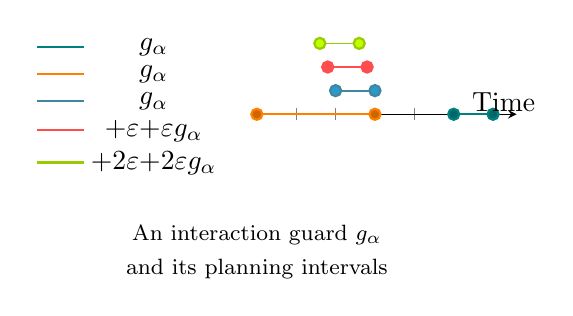
\begin{tikzpicture}[-]
  \begin{axis}[
   axis y line=none,
   y=0.3cm,
   x=1cm,
   xtick={15,15.5,16,...,18},
   restrict y to domain=1:5,
   axis lines=left,
   enlarge x limits=upper,
   cycle list name=exotic,
   scatter/classes={
   o={mark=*}
   },
   scatter,
   scatter src=explicit symbolic,
   every axis plot post/.style={mark=*,thick},
   xlabel=Time,
   x label style={at={(axis description cs:0.95,-0.1)},anchor=south},
   xticklabels={,,},
   legend style={
      draw=none,
      at={(-0.1,-1)},
      anchor=south east
  },
  legend image post style={mark=none}
  ]
  \addplot table [y expr=1,meta index=1, header=false] {
17.5 c
18 c
};\addlegendentry{$g_{\alpha}$}
    \addplot table [y expr=1,meta index=1, header=false] {
15 c
16.5 c
};\addlegendentry{$\backwardp{\hmin}{\hmx} g_{\alpha}$}
\addplot table [y expr=2,meta index=1, header=false] {
16.5 c
16 c
};\addlegendentry{$\backwardp{\hmin}{\hmin}g_{\alpha}$}
\addplot table [y expr=3,meta index=1, header=false] {
16.4 c
15.9 c
};\addlegendentry{$\backwardp{\hmin+\varepsilon}{\hmin+\varepsilon}g_{\alpha}$}
\addplot table [y expr=4,meta index=1, header=false] {
16.3 c
15.8 c
};\addlegendentry{$\backwardp{\hmin+2\varepsilon}{\hmin+2\varepsilon}g_{\alpha}$}
  \end{axis}
  \node (titile)[align=center,yshift=-1.75cm] {\footnotesize An interaction guard $g_{\alpha}$ \\ \footnotesize and its planning intervals};
\end{tikzpicture}
%  \caption{}
  %\captionsetup{justification=centering}
  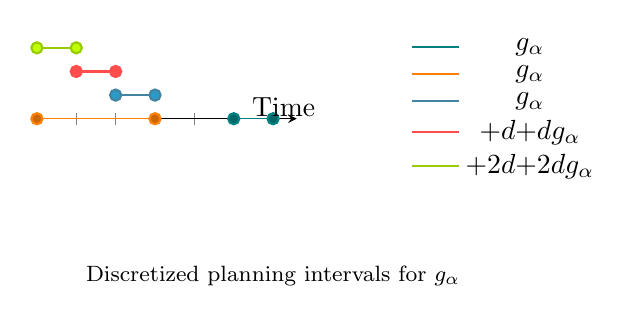
\begin{tikzpicture}[-]
  \begin{axis}[
   axis y line=none,
   y=0.3cm,
   x=1cm,  
   xtick={15,15.5,16,...,18},
   restrict y to domain=1:5,
   axis lines=left,
   enlarge x limits=upper,
   scatter/classes={
   o={mark=*,fill=white}
   },
   scatter,
   cycle list name=exotic,
   scatter src=explicit symbolic,
   every axis plot post/.style={mark=*,thick},
   xlabel=Time,
   x label style={at={(axis description cs:0.95,-0.1)},anchor=south},
   xticklabels={,,},
   legend style={
      draw=none,
      at={(2.2,-1)},
      anchor=south east
  },
  legend image post style={mark=none}
  ]
\addplot table [y expr=1,meta index=1, header=false] {
17.5 c
18 c
};\addlegendentry{$g_{\alpha}$}
\addplot table [y expr=1,meta index=1, header=false] {
15 c
16.5 c
};\addlegendentry{$\backwardp{\hmin}{\hmx} g_{\alpha}$}
\addplot table [y expr=2,meta index=1, header=false] {
16.5 c
16 c
};\addlegendentry{$\backwardp{\hmin}{\hmin}g_{\alpha}$}
\addplot table [y expr=3,meta index=1, header=false] {
16 c
15.5 c
};\addlegendentry{$\backwardp{\hmin+d}{\hmin+d}g_{\alpha}$}
\addplot table [y expr=4,meta index=1, header=false] {
15.5 c
15 c
};\addlegendentry{$\backwardp{\hmin+2d}{\hmin+2d}g_{\alpha}$}
  \end{axis}

  \node (titile)[align=center,yshift=-2cm,xshift=3cm] {\footnotesize Discretized planning intervals for $g_{\alpha}$};
  
\end{tikzpicture}
  %\caption{}
\caption{Discretizing Planning Horizons for Interaction}
\label{fig:disc}
\end{figure*}


\begin{definition}[Planning Timed Automaton]
  \label{def:plan_aut}
  Given n timed components $\tcal{B}_i=(\Loc_i,\loc_0^i,\A_i,\T_i,\X_i,\I_i)$ synchronizing through the interaction set  $\gamma$ such that,
  for each interaction $\alpha\in\gamma$, the guard of $\alpha$ is equal to the guard of one of its included actions.   
  We define the corresponding planning model as the composition of the n timed automata $\tcal{B}_i^p=(\Loc_i^p,\loc_0,\A_i\cup\tcal{P}_i,\T_i^p,\X_i\cup\{x_i^p\},\I_i^p)$,
  w.r.t the interaction set $\gamma\cup\tcal{P}$, where:
  \begin{itemize}
    \item $\tcal{P}_i=\cup_{a\in\A_i} \ p_{a}$ is the set of \emph{Planning Actions}
    \item $\tcal{P}=\{p_{\alpha}=\{p_{a_i}\}_{i\in I}|\alpha\in\gamma\wedge\alpha=\{a_i\}_{i\in I}\}$ is the set of \emph{Planning Interactions}  
    \item $x_i^p$ is a \emph{Tracking Clock} for interactions execution in each component
    \item $\Loc_i^{p}=(\Loc_i\cup\Loc_{i_p})$ is the set of control locations, where $\Loc_{i_p}$ is the set of locations 
      following planning actions
    \item $\T_i^p$ is such that for each $(\loc_i,a_i,g_i,r_i,\loc'_i)\in\T_i$, $a_i\in\alpha$ and for each
      $\delta\in Disc(\alpha)$:
      \begin{itemize}
        \item if $g_{\alpha}\neq\true$ we have:\\
          Planning transitions: $\begin{cases}
            \loc_i\transit{p_{a_i},\true,\emptyset}\loc_{a_i}, \text{ if } g=\true\\
          \loc_i\transit{p_{a_i},\zonep{\delta} g_i,r(x_i^p)}\loc^{\delta}_{a_i}, \text{ otherwise}\end{cases}$\\ 
          Execution transitions: $\begin{cases}
            \loc_{a_i}\transit{a,\true,r_i}\loc'_i, \text{ if } g=\true\\
            \loc_{a_i}^{\delta}\transit{a,g_a\wedge x_i^p=\delta,r_i}\loc'_i, \text{ otherwise}
            \end{cases}$\\
            where $\loc_{a},\loc_{a_i}^{\delta}\in\Loc_{i_p}$.\\
        \item if $g_{\alpha}=\true$, we choose one action $b\in\alpha$:\\
           Planning transitions: $\begin{cases}
            \loc_i\transit{p_{a_i},\true,\emptyset}\loc_{a_i}, \text{ if } a\neq b\\
          \loc_i\transit{p_{a_i},\true,r(x_i^p)}\loc_{a_i}^{\delta}, \text{ otherwise}
           \end{cases}$\\ 
           Execution transitions: $\begin{cases}
            \loc_{a_i}\transit{a_i,\true,r_i}\loc'_i, \text{ if } a\neq b\\
            \loc_{a_i}^{\delta}\transit{a_i,g_i\wedge x_i^p=\delta,r_i}\loc'_i, \text{ otherwise}
            \end{cases}$\\
      \end{itemize}
    \item $\I_i^p$ is the set of \emph{Location Invariants} , such that 
      $\forall\loc_i^p\in\Loc_i^p$, we have:\\
      $\I_i^p(\loc_i^p)= \begin{cases}
        \tpc{}(\loc_i)-\hmin, \text{ if }\loc_i^p=\loc_i\in\Loc_i\\
        x_{i}^{p}\le\delta\wedge\tpc{}(\loc_i), \text{ if } \loc_i^p=\loc_{a_i}^{\delta}\in
        \Loc_{i_p}$ such that $\loc_i\in\Loc_i\wedge\loc_i\transit{p_{a_i}}\loc_{a_i}^{\delta},
      \end{cases}$
  \end{itemize}

\end{definition}

For a composition $\gamma(B_1,\cdots,B_n)$, let $LTS_{p'}=(\Q_{p'},\gamma'\cup\realpos,\lto_{\gamma'})$, where $\gamma'=\gamma\cup\tcal{P}$, be the corresponding labeled transition system of its planning model under the 
standard semantics.  
\begin{theorem}\label{correctness}
  $LTS_{p'}\sqsubseteq_{R'} LTS_g$ where $R'$ is the relation defined as follows:
 
  For $q^p=(\loc^p,\val^p)\in\Q_{p'}$ and $q^g=(\loc^g,\val^g)\in\Q_g$, such that $(q^p,q^g)\in R'$, we have: 

  \begin{itemize}
    \item $\loc^p=(\loc^p_1,\cdots,\loc^p_n),\ \loc_g=(\loc^g_1,\cdots,\loc^g_n)$:
      \[\forall i\in\{1,\cdots,n\},\ \loc^g_i=\begin{cases}
        \loc^p_i, \text{ if } \loc^p_i\in\Loc_i,\\
        \loc_i, \text{ if } \loc^p_i\in\Loc_{i_p}\text{ with }\loc_i\transit{a,g,r}\loc_i^p\in\T_i^p\wedge\loc_i\in\Loc_i,
    \end{cases} 
      \]
      Notice that for the case where $\loc_i^p\in\Loc_{i_p}$, $\loc_i$ is unique by construction of the planning model.
    \item $\val^g=equ(\val^p)$, where $equ(\val^p)$ is the projection of $\val^p$ on clocks of $\val^g$ 
  \end{itemize}
 
  \end{theorem}
  \begin{proof}[Proof of Theorem~\ref{correctness}]
    To prove that $LTS_{p'}\sqsubseteq_{R'} LTS_g$, we need to prove that:

  \begin{enumerate}
    \item $\forall(q^p,q^g)\in R',\sigma\in\gamma\cup\realpos\text{ such that }q^p\transit{\sigma}_{\gamma'}q'^{p}\Rightarrow\exists q'^g.(q'^{p},q'^g)\in R'\wedge 
      q^g\transit{\sigma}_{\gamma}q'^g$
    \item $\forall(q^p,q^g)\in R',p_{\alpha}\in\tcal{P}\text{ such that }q^p\transit{p_{\alpha}}_{\gamma'}q'^{p}\Rightarrow(q'^{p},q^g)\in R'$ 
  \end{enumerate}

  \begin{enumerate}
    \item
  \begin{enumerate}
    \item Suppose that $(q^p,q^g)\in R',\sigma=\alpha\in\gamma$ and $q^p\transit{\alpha}_{\gamma'}q'^{p}$ with $q'^p=(({\loc'}_1^p,\cdots,{\loc'}_n^p),{\val'}^p)$. We have:
      $q^p\transit{\alpha}_{\gamma'}q'^{p}\Rightarrow g_{\alpha}$ is $\true$, and for 
      $\alpha=\{a_i\}_{i\in\I}$, by construction of the planning automaton, we have:
      $\loc_i^g\transit{a_i,g_i,r_i}{\loc'}_i^g$ such that ${\loc'}_i^g={\loc'}_i^p$. Moreover, 
     since the same clocks are reset by the execution of $\alpha$ in both models, we deduce that $\val'^g=equ(\val'^p)$. 
      By remarking that the state of components not participating in $\alpha$ remains the same, we conclude that $\exists {q'}^g$ such that 
      $q^g\transit{\alpha}_{\gamma}{q'}^g\wedge({q'}^p,{q'}^g)\in R'$. 
    \item Suppose that $(q^p,q^g)\in R',\sigma\in\realpos$ and $q^p\transit{\sigma}_{\gamma'}
      q'^{p}$. For $q^p_i=(\loc_i^p,\val_i^p)$, we define $\I_g$ the set of indexes such that 
       $\loc_i^p\in\Loc_i$, and $\I_p$ the set of indexes such that $\loc_i^p\in\Loc_{p_i}$. 
       \begin{itemize}
         \item $\forall i\in\I_g$.$\loc_i^p=\loc_i^g\wedge\q_i^p\transit{\sigma}
           {q'}_i^p\Rightarrow q_i^g\transit{\sigma}{q'}_i^g$. This implication is a direct result of the planning model definition since: $\sigma\le\I(\loc_i^p)\le\tpc{}(\loc_i^g)-\hmin$.
           
         \item $\forall i\in\I_p.\loc_i^g=\loc_i$ such that $\loc^p_i\in\Loc_{i_p}\text{ with }\loc_i\transit{a,g,r}\loc_i^p\in\T_i^p\wedge\loc_i\in\Loc_i$.
           Thus $\q_i^p\transit{\sigma}{q'}_i^p\Rightarrow q_i^g\transit{\sigma}{q'}_i^g$, since $\I(\loc_i^p)\implies\tpc{}(\loc_i^g)$.

         \end{itemize}
       We conclude that $\exists q'^g$ such that $q^g\transit{\sigma}_{\gamma}{q'}^g\wedge({q'}^
         p,{q'}^g)\in R'$.
  \end{enumerate}

\item Suppose that $(q^p,q^g)\in R'$ and $q^p\transit{p_{\alpha}}_{\gamma'}q'^{p}$, with 
  $p_{\alpha}\in\tcal{P}$ and $q'^p=(({\loc'}_1^p,\cdots,{\loc'}_n^p),{\val'}^p)$. We have:
      $q^p\transit{p_{\alpha}}_{\gamma'}q'^{p}\Rightarrow$ for $\alpha=\{a_i\}_{i\in\I}$
      $\loc_i^g=\loc_i^p\wedge\loc_i^g\transit{p_{a_i}}{\loc'}_i^p$. Moreover, since planning
      actions reset only the clocks $x_i^p$ for tracking execution time, we can deduce that
      $({q'}^p,q^g)\in R'$.
  \end{enumerate}

\end{proof}

Once interactions planning encoded, one last thing to do is to add the set of bad states to each
planning automaton (if needed) and find a strategy to avoid those states. 
Figure~\ref{fig:task} depicts the corresponding planning automaton for a task
component of the running example w.r.t Definition~\ref{def:plan_aut}. Here, $x_p$ is the clock
used for tracking the execution date of an interaction within the task component.
Locations suffixed by \emph{p}, correspond to locations following 
planning actions, whereas locations ending with \emph{err} define the bad states, that is,
states with urgent time progress condition(s) and no possible execution removing the urgency. In this example, we put $\hmin = 2$. 

For a matter of simplicity, we restrict the planning horizon values
by putting for each interaction $\alpha\in\gamma/ \hmx=h_{\min}$.
Notice that in this case,
the method checks if a given system is deadlock-free when being planned with
a $h_{\min}$ horizon.
\begin{figure}[h]
  \centering
  \includegraphics[scale=0.4]{../images/task}
  \caption{Planning automaton for the task component}
  \label{fig:task}
\end{figure}

\subsection{Discussion}

In this section, we explained how the problem of planning interactions can be formalized into
a real-time controller synthesis approach. However, this approach has some drawbacks.
In order to encode planning of interactions in components as timed automata, this approach
restricts its scope to discretized horizon values which results in having less control
over the planning dates of interactions, and leads in case of a high number of discretized values,
to an explosion in the number of planning transitions. 
Additionally, it considers only a class of systems where interactions have timing constraints on 
up to one of their participating components action. Otherwise, the planning should be encoded
on the composition, which represents a tedious work. 

\section{Communication Delays}
\section{Local Planning Semantics}
\section{Correctness}







